
\begin{table}[b]
% \captionsetup{   font = {scriptsize},  }
 \caption{Dataset properties. For each dataset,  we specify whether the attributes have Boolean or categorical domains, the number of tuples and attributes, and the average number of distinct values per attribute}
 \label{table:dataset_description}
%\scalebox{.9}{
\begin{tabular}{lcrrr}
\textbf{Dataset} & \textbf{Attributes} & \textbf{\# tuples} & \textbf{\# attributes} & \textbf{Avg \# values per attribute}  \\
Animals          & Boolean         &  $50$  &  $85$  &  2  \\
Solar flare      & categorical &  $1\,389$  &  $11$  &  $3.3$  \\
Tic-tac-toe      & categorical  &  $958$  &  $10$  &  $2.9$  \\
Nursery          & categorical &  $12\,960$  & $8$  &  $3.4$  \\
Voting           & categorical &  $435$  &  $17$  &  $3.0$  \\
Chess (Kr-vs-Kp) & categorical &  $3\,196$  &  $36$  &  $2.1$  \\ 
Mushroom         & categorical &  $8\,124$  &  $22$  &  $5.6$
\end{tabular}
%}
\end{table}

The main goal of this section is to evaluate whether ReDF problems can be solved using a generic solver. In particular, we focus on solving the problem formulations as we specified them in ASP. We investigate whether the problems can be solved, and for a number of tasks compare the results and runtimes to those obtained by specialized algorithms. Since we here use generic problem formulations and generic solvers that have neither been designed nor optimized for the tasks under consideration, we cannot expect the approach to be as efficient as specialized algorithms. However, what is more important is that we demonstrate that all tasks formalized and prototyped using the ReDF framework can be solved using a unified approach.


\textit{Experimental setup and datasets.} The ASP engine we use is 64-bit clingo (clasp with the gringo grounder) version 3.0.5 with the parameter \texttt{--heuristic=Vmtf} (see Appendix \ref{subsec:evaluatingsolver} for details on the parameters) and all experiments are executed on a 64-bit Ubuntu machine with Intel Core i5-3570 CPU @ 3.40GHz x 4 and 8GB memory, except for Maximum $k$-tiling on Chess and Mushrooms datasets where Intel Xeon CPU with 128GB of memory (all single-threaded) has been used due to high memory requirements. For most experiments we use the datasets summarized in Table \ref{table:dataset_description}, which all but one originate from the UCI Machine Learning repository \citep{ucidatasets}. The \emph{Animals (with Attributes)} dataset was taken from \cite{animalDataset}. For the purely relational factorization task, the data and experiment results are described separately in the corresponding subsection. 

In Subsection~\ref{subsec:solvingexisting} we show how ReDF formulations of existing data mining tasks (from Section~\ref{section:dm_problems}) can be solved using the implementation presented in Section~\ref{section:implementation}, afterwards in Subsection~\ref{subsec:solvingrelational} we show the results of the purely relational data factorization task. The ASP solver parameters used in the experiments and a breakdown of individual solving steps and their runtimes determined by the meta-experiment are presented in Appendix~\ref{subsec:evaluatingsolver}.

\subsection{Solving existing tasks}
\label{subsec:solvingexisting}
\paragraph{Maximum $k$-Tiling in Categorical Data}
\begin{table}[t]
\captionsetup{
    font = {small},
  }
\begin{center}
\caption{Maximum $k$-Tiling}
\label{tab:tiling}
\begin{subtable}{.45\textwidth}
\captionsetup{
    font = {small},
  }
\caption{Runtime}
\label{tab:tiling:time}
\scalebox{.75}{
\begin{tabular}{lrrrrr}
  \phantom{Dataset} & \multicolumn{5}{c}{\textbf{Number of tiles ($k$)}}\\
\textbf{Dataset} & \textbf{5} &    \textbf{10} &   \textbf{15} &  \textbf{20} & \textbf{25} \\ \hline
Animals    &36s  & 1m4s  &  1m21s  &  1m32s  & 1m36s \\
Solar flare&6s   & 10s  &  13s  &  16s  & 18s \\
Tic-tac-toe&22s  & 31s  &  33s  &  34s   & 35s \\
Nursery    &4m19s & 6m32s &  7m32s &  7m56s & 8m13s \\
Voting     &52s  &  1m28s &  1m42s &  1m46s & 1m49s \\
Chess      &17h03m & 22h31m & - & - & -\\
Mushroom &13h09m & 19h44m & - & - & -\\
\end{tabular}
}
\end{subtable}
\hfill
\begin{subtable}{.41\textwidth}
\captionsetup{
    font = {small},
  }
\caption{Coverage}
\label{tab:tiling:coverage}
\scalebox{.75}{
\begin{tabular}{rrrrr}
  \multicolumn{5}{c}{\textbf{Number of tiles ($k$)}}\\
\textbf{5} &    \textbf{10} &   \textbf{15} &  \textbf{20} & \textbf{25} \\ \hline
0.327 & 0.472 & 0.573 & 0.649 & 0.709\\
0.416 & 0.565 & 0.655 & 0.721 & 0.751\\
0.251 & 0.449 & 0.623 & 0.784 & 0.907\\
0.269 & 0.454 & 0.634 & 0.773 & 0.905\\
0.399 & 0.553 & 0.662 & 0.749 & 0.810\\
0.483 & 0.618 &- &-   &-\\
0.476 & 0.586 &-   &- &-
\end{tabular}
}
\end{subtable}
\end{center}
\end{table}


\label{subsec:experiments_tiling}

We first consider the Maximum $k$-Tiling problem from Section \ref{subsection:tiling} and present timing and coverage results in Table~\ref{tab:tiling} obtained on all datasets from Table \ref{table:dataset_description}.

In all cases the problem specification given in Listing~\ref{lst:encoding} was used to greedily mine $k=25$ tiles. Since the problem becomes more constrained as the number of tiles increases, runtime decreases for each additional tile mined. We therefore report total runtime and coverage for different values of $k$, i.e., for different total numbers of tiles. Only $k=10$ tiles were mined on Chess and Mushroom due to long runtimes.


\textit{Effect of sampling~}As we can see from Table~\ref{tab:tiling:time}, runtimes are quite long on datasets like Mushroom. To address this issue, we use the sampling procedure of Algorithm~\ref{sampling} with the following parameters: $\alpha = 0.4$ and $N = 20$, i.e., 40\% of all attributes were selected uniformly at random for each sample and 20 samples were used. Intuitively, the larger the sample size and the more samples, the better we approximate the exact result.

With the given parameters, we attain an order of magnitude improvement in runtime: instead of 19 hours with the regular algorithm, using sampling it takes only one hour to compute 10 tiles as indicated in Figure \ref{fig:tiling_time_comparison}. The effect of using sampling on coverage can be seen in Figure~\ref{fig:tiling_comparison}: the first tiles that are mined have lower coverage than when sampling is not used, but after a while the difference in coverage with LTM-k remains more or less constant and even slightly decreases. LTM-k is the original, specialized tiling algorithm, to which we compare next.


\textit{Comparison to a specialized algorithm~}We now compare the performance of the ASP-based implementation of LTM-k greedy strategy to that of a specialized implementation\footnote{\url{http://people.mmci.uni-saarland.de/~jilles/prj/tiling/}}. Figures~\ref{fig:tiling_time_comparison} and~\ref{fig:tiling_comparison} present both runtime and coverage comparisons obtained on Mushroom, both for our approach (with and without sampling) and the specialized miner. 

Without sampling, we can see that our approach gives the same results in terms of the coverage as the LTM-k algorithm. This is as expected though, since both LTM-k and our approach guarantee to find an optimal solution in each iteration. \changesb The slight difference between the two coverage curves in Figure \ref{fig:tiling_comparison} is caused by the fact that multiple tiles can have the same (maximum) area, and some choice between those has to be made. Although these choices are typically made deterministically, the different implementations make decisions based on different criteria, resulting in slightly different tilings. \changese

Unfortunately, the ASP solver is not as efficient as the specialized miner as can be seen in Figure \ref{fig:tiling_time_comparison}, and the generality of the approach comes at the cost of longer runtimes. However, as already discussed, using a sampling approach can substantially decrease the runtime. Experiments on other datasets showed similar behavior to that depicted here.

\begin{figure}[t]
      \captionsetup{
                   skip=-2pt
                 }
  \begin{center}
    \begin{subfigure}{.49\textwidth}
      \captionsetup{
                   font={scriptsize},
                   skip=-5pt
                 }
      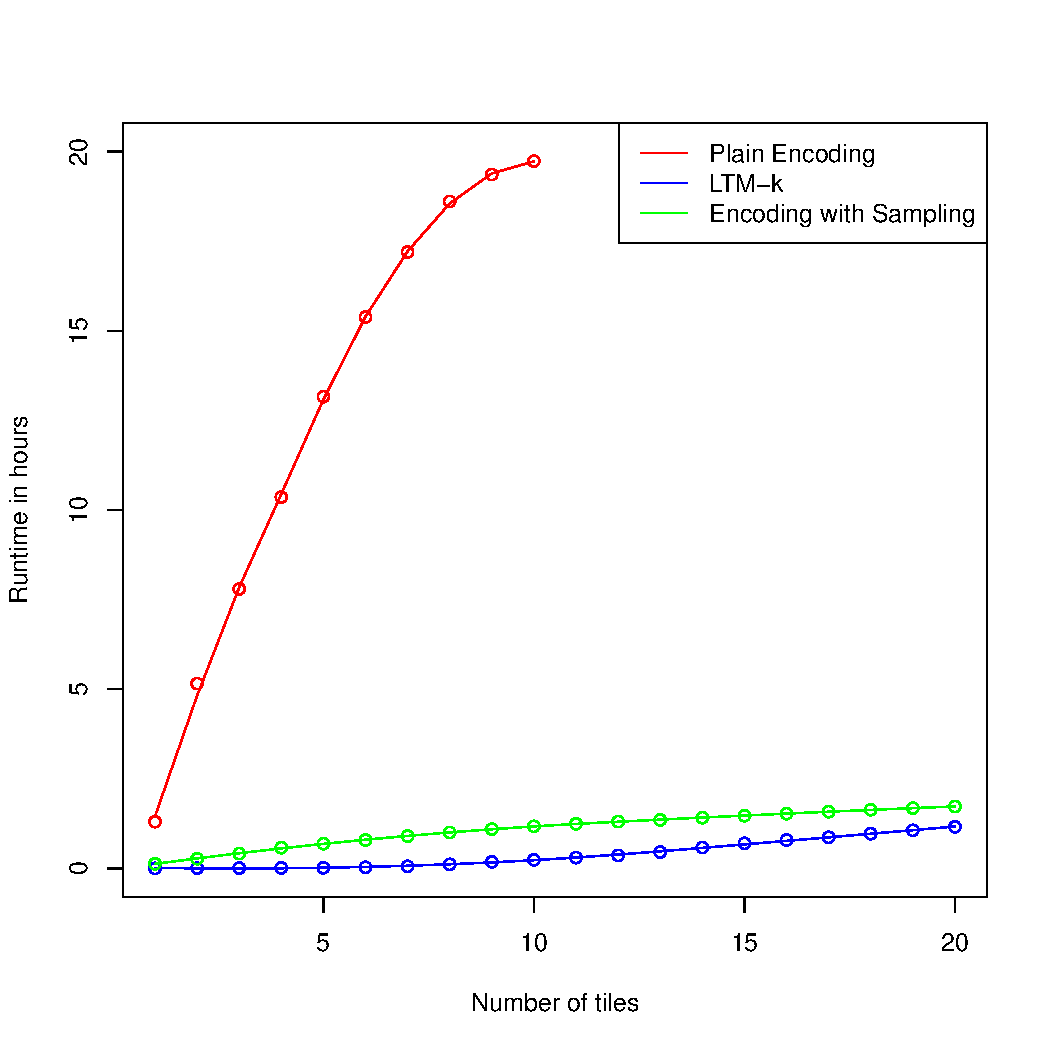
\includegraphics[width=\textwidth]{tiling-time-plot.pdf}
      \caption{Runtime}
      \label{fig:tiling_time_comparison}
    \end{subfigure}
    \hfill 
    \begin{subfigure}{.49\textwidth}
      \captionsetup{
                   font={scriptsize},
                   skip=-5pt
                 }
      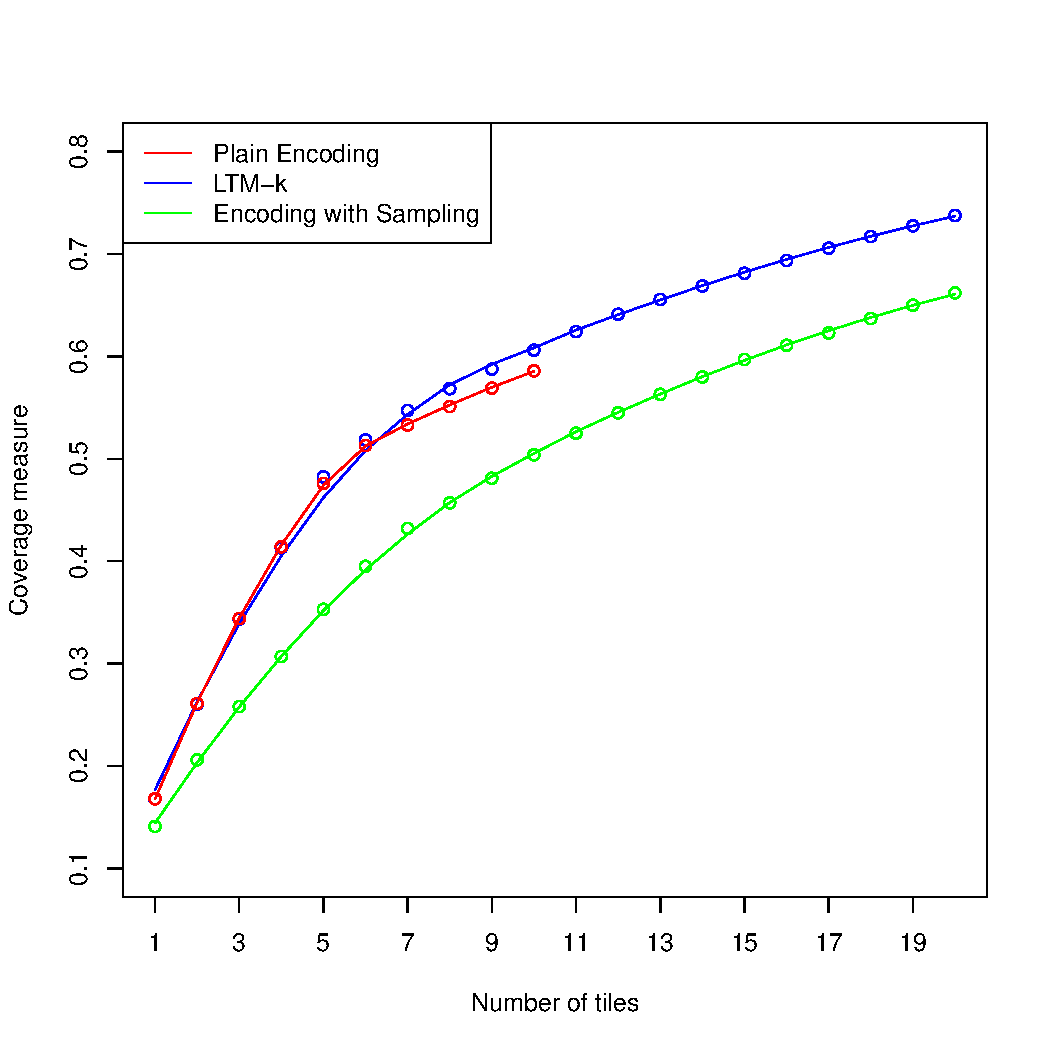
\includegraphics[width=\textwidth]{tiling_comparison.pdf}
      \caption{Coverage}
      \label{fig:tiling_comparison}
    \end{subfigure}
  \caption{Tiling comparison (runtime, coverage) with LTM-k (Mushroom dataset)}
  \end{center}
\end{figure}

\paragraph{Overlapping tiling}
To evaluate the overlapping tiling task from Subsection \ref{subsubsec:overlapping_tiling}, we apply the model in Listing~\ref{encoding_noisy} (ASP encoding in Appendix \ref{ASP_appendix}) to the five smaller datasets from Table \ref{table:dataset_description}. We experiment with two levels of overlap, i.e., parameter $N$ is set to either 1 or 2: tiles can intersect on at most one or two attribute(s). As the results in Table~\ref{tab:overlapping} show, allowing limited overlap can lead to a small increase in coverage, but runtimes also increase due to the costly aggregate operation in Line~\ref{line_intersect_count} of Listing~\ref{encoding_noisy}. 

However, what is important to emphasize here is that only a small change in the problem formalization is sufficient to allow for overlap in the tilings, while the solver can still solve the problem without any further changes. And although the runtimes are longer when more overlap is allowed, the difference with the basic, non-overlapping setting is moderate.

\begin{table}[t]
\captionsetup{
    font = {small},
  }
\begin{center}
\caption{Maximum $k$-Tiling with overlap. The maximal allowed overlap is limited by parameter $N$}
\label{tab:overlapping}
\begin{subtable}{.36\textwidth}
\caption{Runtime}
\label{tab:overlapping:time}
\scalebox{.75}{
\begin{tabular}{lcrrrrrr}
\phantom{Dataset}     & \multicolumn{5}{c}{\textbf{Number of tiles ($k$)}}\\
\textbf{Dataset}      &  \textbf{N} &  \textbf{5} &    \textbf{10} &   \textbf{15} &  \textbf{20} & \textbf{25} \\ \hline
Animals               & 1 & 1m10s &2m28s&3m46s&4m24s &4m47\\
\phantom{Animals}     & 2 & 1m39s &4m10s&6m26s  &7m40s&8m10s\\
Solar flare           & 1 & 8s  &13s &17s   &21s &24s\\
\phantom{Solar flare} & 2 & 8s  &15s &20s   &25s &29s\\
Tic-tac-toe           & 1 & 24s &41s &49s   &52s &53s\\
\phantom{Tic-tac-toe} & 2 & 23s &43s &51s   &55s &56s\\
Nursery               & 1 & 5m00s&8m19s&10m10s  &10m48s&11m12s\\
\phantom{Nursery}     & 2 & 5m43s&9m32s&11m9s&11m50s&12m12s\\
Voting                & 1 & 1m10s &2m19s& 2m53s &3m8s&3m15s\\
\phantom{Voting}      & 2 & 1m39s &3m34s& 4m35s &5m9s&5m33s
\end{tabular}
}
\end{subtable}
\hfill
\begin{subtable}{.37\textwidth}
\caption{Coverage}
\label{tab:overlapping:coverage}
\scalebox{.75}{
\begin{tabular}{rrrrr}
\multicolumn{5}{c}{\textbf{Number of tiles ($k$)}}\\
\textbf{5} &    \textbf{10} &   \textbf{15} &  \textbf{20} & \textbf{25} \\ \hline
0.327&0.475&0.583&0.663&0.722\\
0.332&0.482&0.592&0.675&0.742\\
0.433&0.595&0.684&0.734&0.756\\
0.452&0.602&0.685&0.731&0.755\\
0.253&0.451&0.626&0.781&0.898\\
0.253&0.451&0.626&0.781&0.898\\
0.268&0.454&0.633&0.772&0.905\\
0.268&0.454&0.633&0.772&0.905\\
0.403&0.558&0.675&0.765&0.828\\
0.409&0.571&0.683&0.762&0.819
\end{tabular}
}
\end{subtable}
\end{center}
\end{table}

\paragraph{Boolean matrix factorization (BMF)}
We perform Boolean matrix factorization (Section \ref{subsection:bmf}) by applying the formalization of Listing~\ref{bmf} and compare the results to those obtained by ASSO\footnote{\url{http://www.mpi-inf.mpg.de/~pmiettin/src/DBP-progs/}} \citep{conf/icdm/Miettinen12} with the no-overcoverage flag (\texttt{-P1000}). The factorization rank $k$ is incremented by one in each iteration, and meanwhile coverage gain and runtime are measured. The results for Animals are presented in Figure~\ref{figure:bmf} and show that coverage is almost identical to that obtained by ASSO. Again, this is unsurprising, as our implementation follows the same solving strategy.  However, runtimes are several times higher, which is due to the usage of a general solver that is not optimized for this type of task. Results obtained on other datasets are very similar and are therefore not presented here.

\begin{figure}
%  \vspace{-3mm}
\begin{center}
\begin{subfigure}{.49\textwidth}
\centering
\captionsetup{skip=-3pt}
  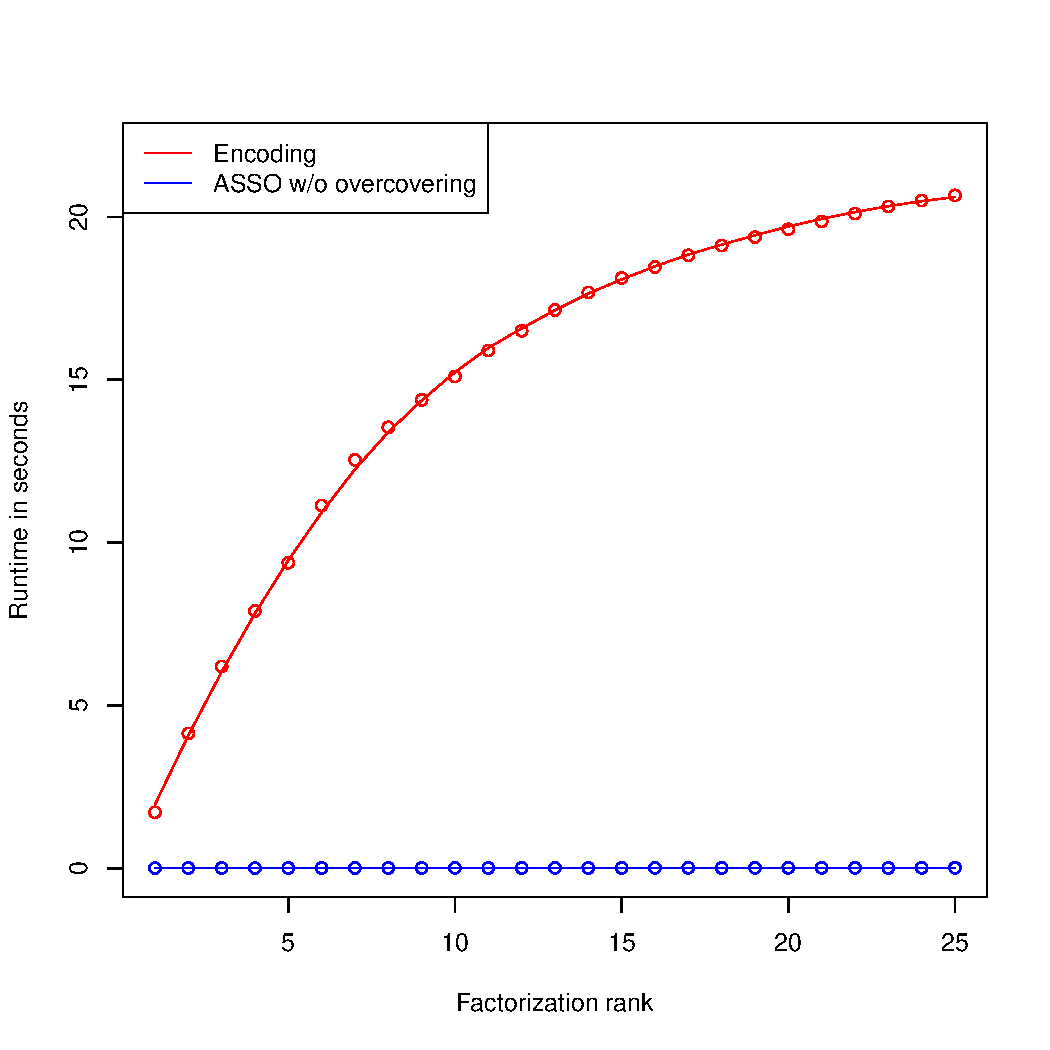
\includegraphics[width=\textwidth]{decomposition_time.pdf}
\caption{Runtime}
\end{subfigure}
   \hfill 
\begin{subfigure}{.49\textwidth}
\centering
\captionsetup{skip=-3pt}
  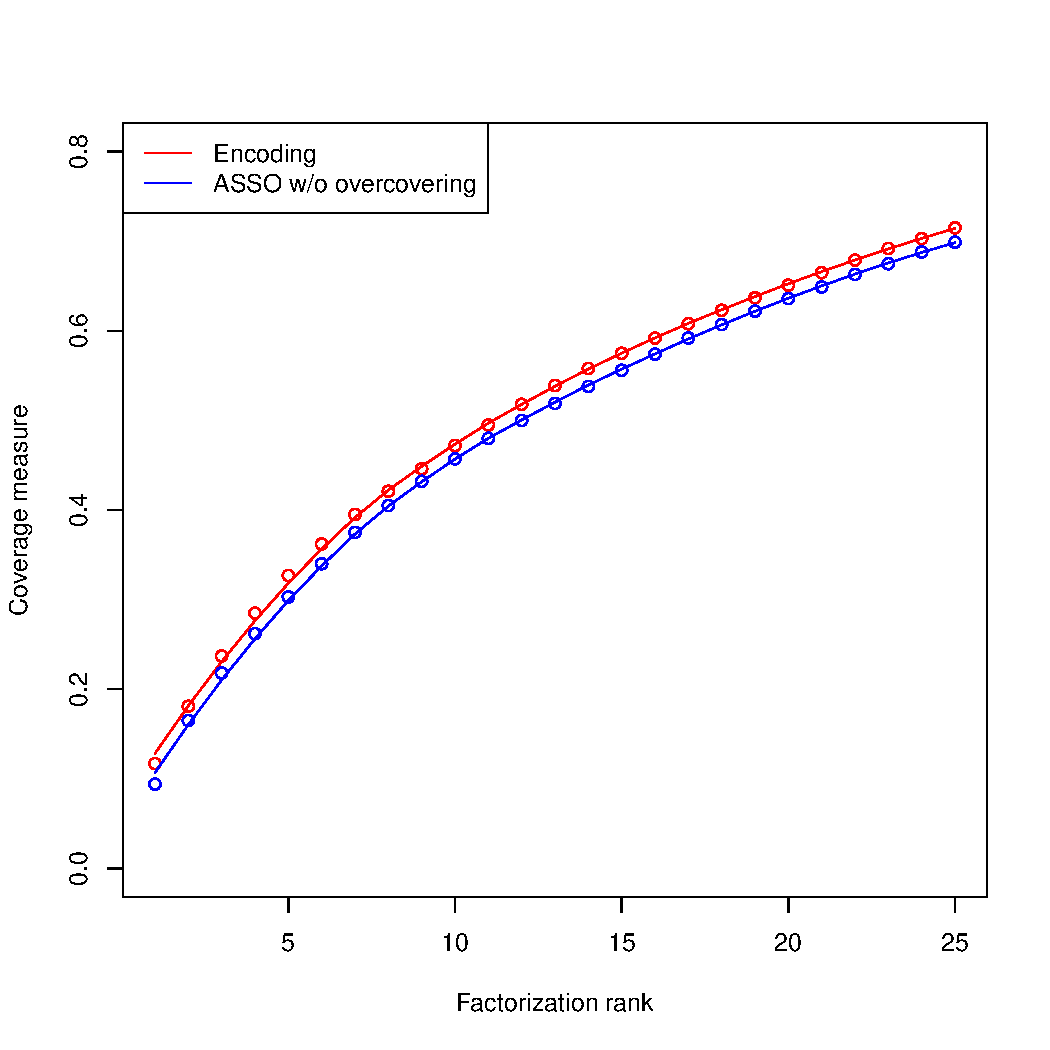
\includegraphics[width=\textwidth]{decomposition_coverage.pdf}
\caption{Coverage}
\end{subfigure}
  \captionsetup{skip=2pt}
  \caption{Boolean matrix factorization on datasets Animals. Runtime and coverage are depicted for different factorization ranks.}
  \label{figure:bmf}
  \end{center}
  \end{figure}

\paragraph{Discriminative pattern set mining}

\begin{figure}[thb]
\begin{subfigure}{.56\textwidth}
  \captionsetup{skip = 0pt}
\begin{center}
  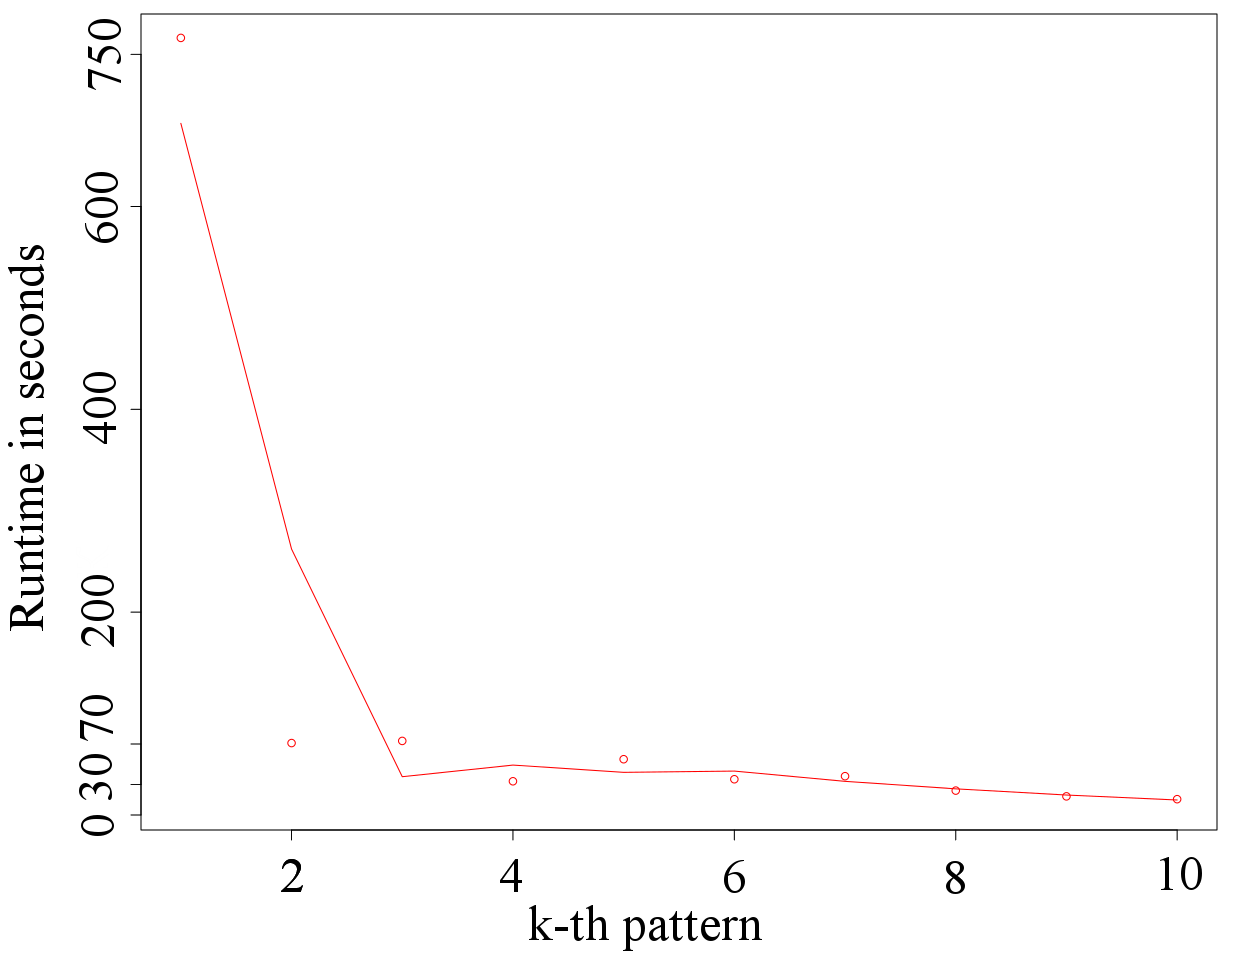
\includegraphics[width=0.9\linewidth]{DiscriminativeChess.png}
  \caption{Runtime (in s) to mine $k$-th discriminative pattern on Chess dataset ($\alpha = 1$, i.e., positive and negative tuples are weighted equally)}
  \label{figure:discriminative_chess}
 \end{center}
\end{subfigure}
\begin{subfigure}{.43\textwidth}
\begin{center}
\captionsetup{skip = 0pt, font=small}
\captionof{figure}{Discriminative mining coverage on Chess and Tic-tac-toe datasets ($\alpha = 1$, i.e., positive and negative tuples are weighted equally)}
\label{table:discriminative_results}
  \scalebox{0.8}{
\begin{tabular}{lll}
  \phantom{Negative }  & Tic-tac-toe ($k$ = 5) & Chess ($k$ = 10) \\ \cline{2-3} \vspace{-8pt}\\
  Covered  $-$              & 92 (27.7\%)           & 160 (7\%)        \\
  Covered  $+$              & 626 (100\%)           & 864 (95.5\%)     \\
  Difference                & 534                   & 704              \\
  Runtime                   & 0.52s                 & 18m48s           
 \end{tabular}
 }
\end{center}
\end{subfigure}
\caption{Discriminative pattern set mining summary: runtime (left) and coverage (right)}
\end{figure}

\begin{figure}[thb]
\begin{center}
\begin{subfigure}{.49\textwidth}
  \captionsetup{skip = -3pt}
  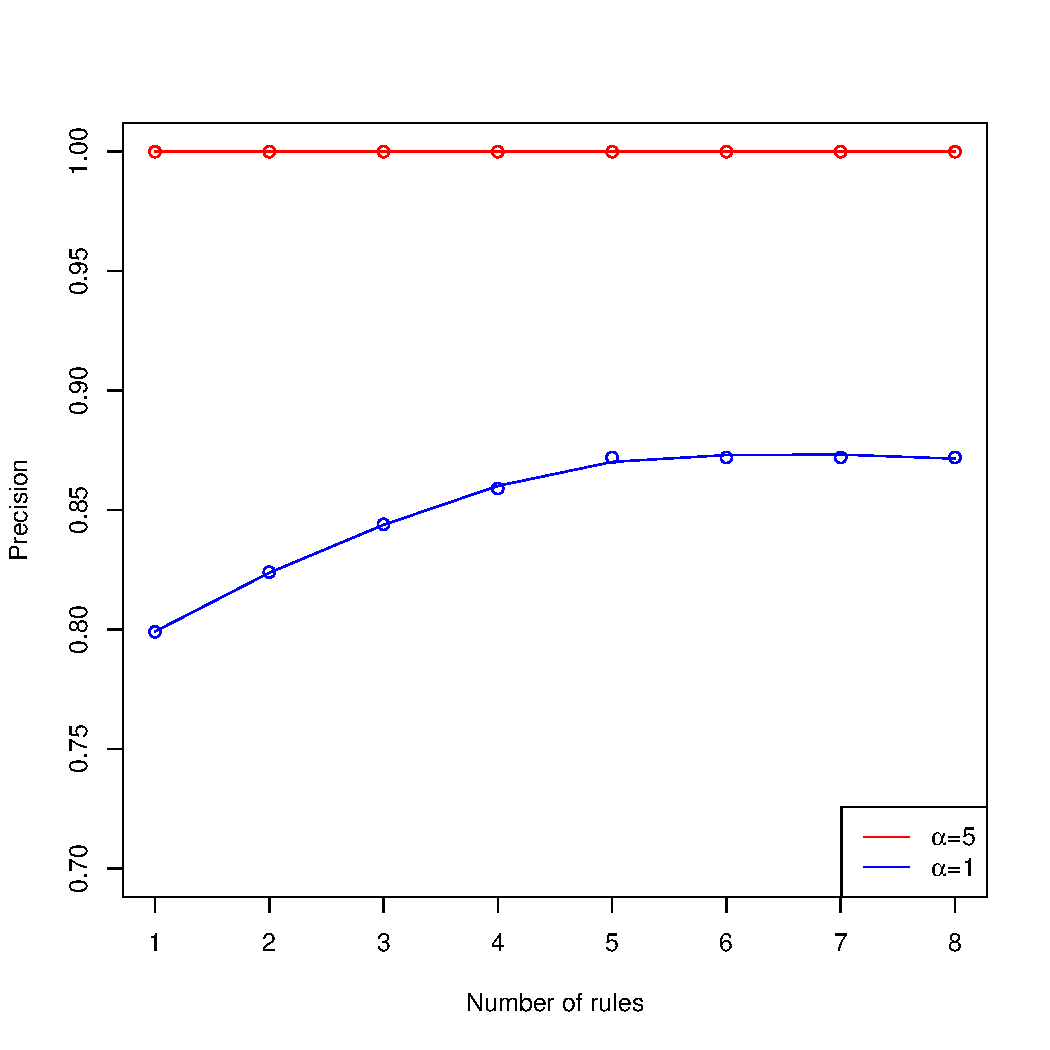
\includegraphics[width=\textwidth]{discriminative_precision.pdf}
  \caption{Precision}
\end{subfigure}
   \hfill 
\begin{subfigure}{.49\textwidth}
  \captionsetup{skip = -3pt}
  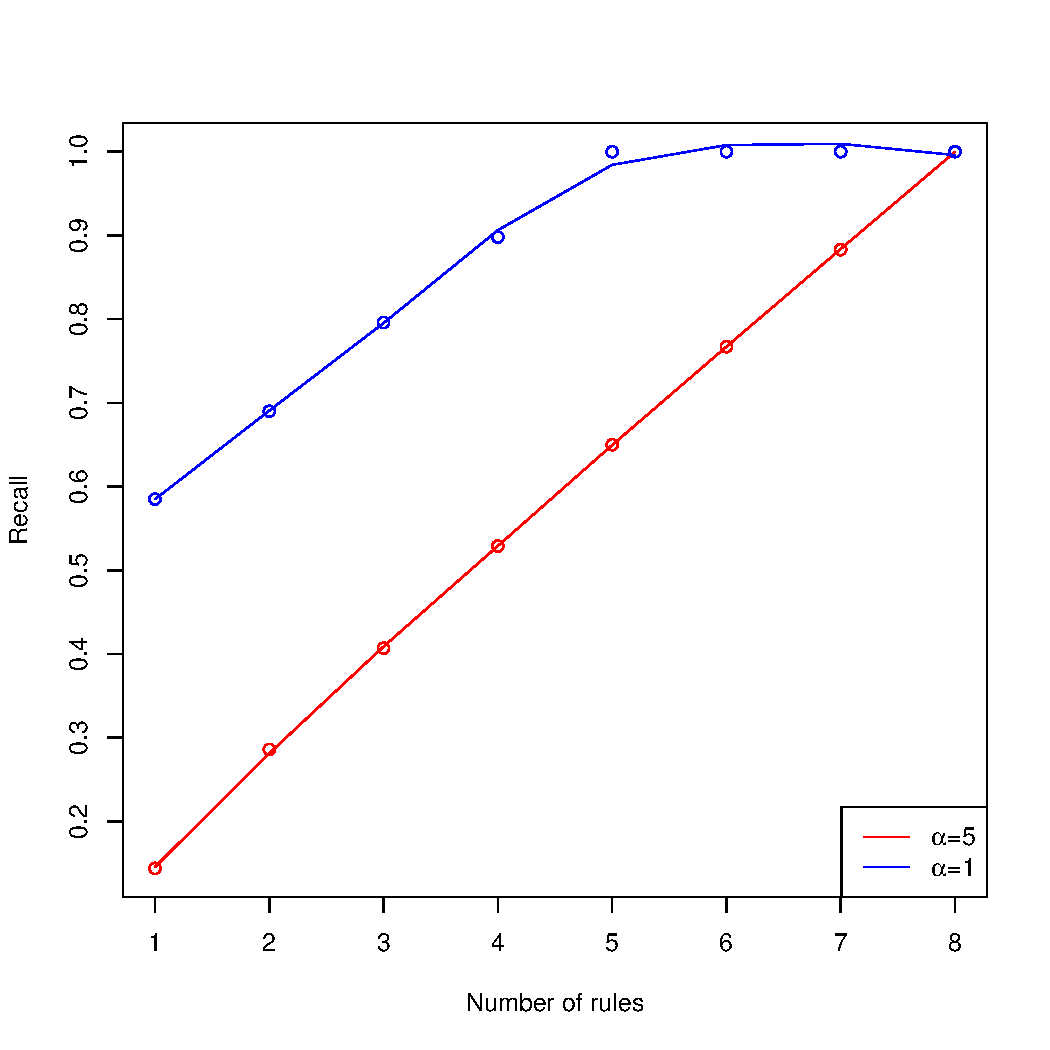
\includegraphics[width=\textwidth]{discriminative_recall.pdf}
  \caption{Recall}
 \end{subfigure}
 \end{center}
  \captionsetup{skip = -4pt}
  \caption{Discriminative pattern set mining (Tic-tac-toe dataset): precision (left) and recall (right) for different $\alpha$, i.e., for varying weights of covering  negative transactions}
  \label{fig:discriminative_precision_recall}
\end{figure}
 Here we demonstrate how the discriminative $k$-pattern mining model from Section \ref{subsec:discriminative} can be solved. For this we use Chess and Tic-tac-toe from Table \ref{table:dataset_description}, each of which has a binary class label indicating whether a game was won or not and can therefore be naturally used for this task. 

We apply the encoding from Listing~\ref{encoding_discriminate} to both datasets, set $\alpha = 1$ to weigh positive and negative tuples equally, and summarize the results in Figure~\ref{table:discriminative_results}. The results show that five patterns suffice to cover all positive examples of Tic-tac-toe, hence mining more than five patterns would be useless. 92 of the 718 covered tuples are negative, i.e., $12.8\%$, while $34.7\%$ of the tuples in the complete dataset is negative. For Tic-tac-toe, the time needed to solve this task is very limited: about half a second.

Figure~\ref{figure:discriminative_chess} shows the runtime needed to iteratively find subsequent patterns in the Chess dataset. Interestingly, it seems that the problem becomes substantially easier (computationally) once the first few patterns have been found: the runtime per pattern drops heavily. This confirms that the search space shrinks when the problem becomes more constrained, i.e., the number of answer sets decreases with the addition of more constraints.

We next show the influence of the $\alpha$ parameter, i.e., the relative weight of covering positive and negative tuples in the optimization criterion. By increasing $\alpha$, the `penalty' for covering a negative tuple is increased and the algorithm can be forced to select more conservative rules. We investigate the effect of this parameter by measuring and comparing precision and recall of the obtained pattern sets for $\alpha = 1$ and $\alpha = 5$. Figure~\ref{fig:discriminative_precision_recall} shows that precision goes to $1$ when $\alpha$ is increased, while recall is decreased but this can be compensated by mining a larger number of patterns\footnote{\changesb Appendix \ref{appendix:precision_recall} presents the data points of Figure \ref{fig:discriminative_precision_recall} as a traditional precision-recall plot.\changese}.

This task differs from the previous one in its optimization criterion: positive coverage penalized by negative coverage allows for fast inference and discovery of the optimal solution, which results in shorter runtimes than for tiling. 

\paragraph{Matrix block-diagonal form}

We apply three versions of the encoding to the Animals dataset \citep{animalDataset}. The results presented in Figure~\ref{fig:diag_examples} demonstrate that the Animals dataset can be re-arranged into block-diagonal form using our proposed framework. The runtime in all experiments are on the order of seconds. Parameters used in the experiments were $\alpha=\frac{3}{20}$ and $\beta=\frac{1}{20}$. Figure \ref{fig:noisy_block_diagonal} demonstrates the model from Section \ref{subsec:blockdiagonal}, with the same $\alpha$, $\beta$ and $N=1$. The low-level encoding of this model is given in Listing \ref{lst:diag_encoding}.

\subsection{Purely relational data factorization}
\label{subsec:solvingrelational}

\begin{figure}[tbh]
  \centering
  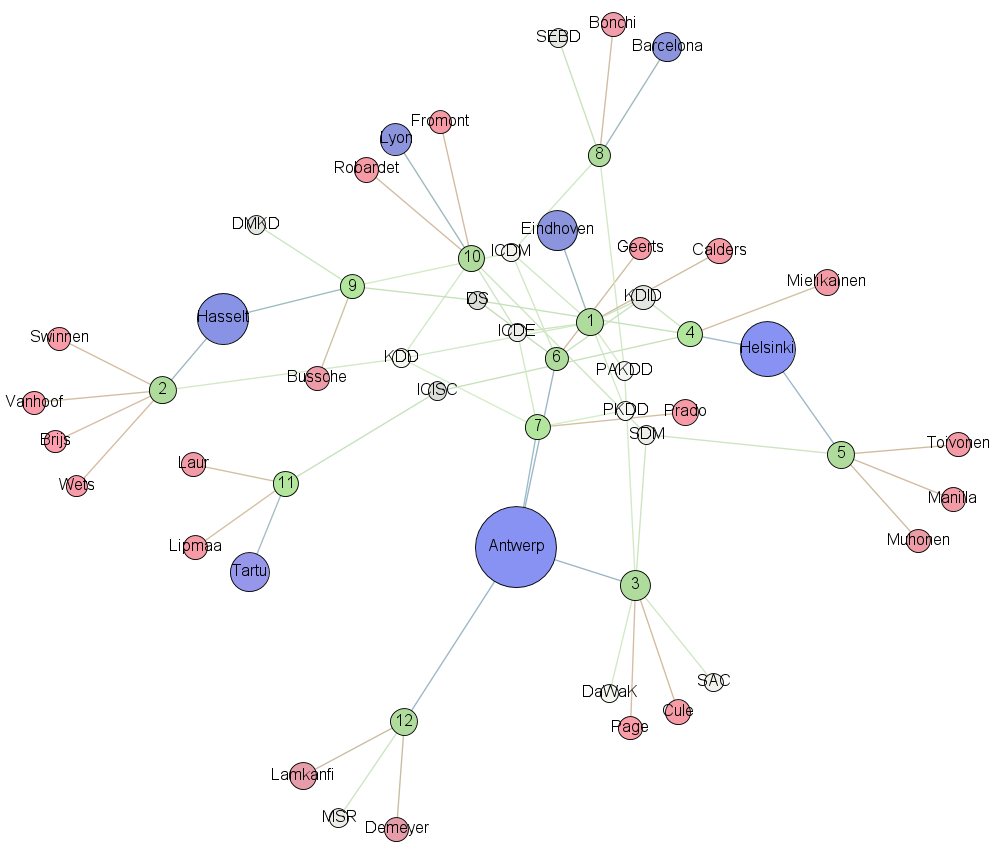
\includegraphics[width=1.00\linewidth]{Bart_clustering.png}
  \captionsetup{skip=-0pt}
  \caption{Clustering in topics by ReDF. Red nodes represent co-authors, blue their university cities, white nodes venues and green topics that bind them  together. If there is an edge between a topic and a node, then there is a corresponding element in the relation (i.e., \textit{interestedIn}, \textit{specializedIn} or \textit{inField}) }
  \label{figure:purely_relational_decomposition}
\end{figure}

In Section~\ref{sec:pure_decomposition} we described how to model the factorization of \textit{publishedIn(Author, University, Venue)} into three binary relations with a latent variable \textit{Topic}. We now evaluate whether the standard ASP solver can solve this task. Unfortunately, we cannot expect a generic solver to handle enormous datasets such as the one from ArXiv as described by \cite{Gopalan2013Efficient}. Instead, we demonstrate a proof-of-concept of solving the model in Listing~\ref{lst:pure_relational_encoding} on a moderate dataset.

We constructed a dataset for a well-known colleague from the data mining community: Bart Goethals (Antwerp University). We collected his publication list from Microsoft Academic Search\footnote{\scriptsize{\url{http://academic.research.microsoft.com/Author/2266478/bart-goethals}}} and extracted for each paper the publication venue, and all co-authors together with their corresponding affiliations (i.e., the last known affiliation for each author in this list of papers). Each unique combination of venue, co-author, and affiliation resulted in a tuple in the \textit{publishedIn} relation. The complete dataset contains 57 tuples over 19 universities, 38 authors, and 15 venues.

Intuitively, if a set of \emph{authors} from a set of \emph{universities} publish in a set of \emph{venues}, then there must be an underlying research \emph{topic} that unites them. Hence, by factorizing the relation into three separate relations, we cluster each of the entity types into a (fixed) number of topics, as indicated by the value of the latent \textit{Topic} variable.

The results for factorization using $K = 12$ topics and $\alpha=\frac{1}{2}$ are presented in Figure~\ref{figure:purely_relational_decomposition}, including co-authors (red), universities (blue), publication venues (purple), and topics (green). To determine the number of topics $K$, we tracked the optimization criterion while increasing $K$ and stopped when this no longer improved.

Since the task is of an exploratory character, we can only qualitatively evaluate the results. We observe that all data mining venues are located together in the center, connected to the same topics. SEBD, an Italian database conference, stands apart, and there is also a separate block for database and computing venues DaWaK and SAC. \changesb Manual inspection of the results indicates the topics (or clusters) to be coherent and meaningful: they represent different affiliations and groups of co-authors that Bart Goethals has collaborated with. For example, topic $5$ contains the SDM conference, the University of Helsinki, and three co-authors specialized in Data Mining. Hence, this topic could be described as ``Data mining collaboration with the University of Helsinki'', which makes perfect sense as Bart Goethals was previously a researcher in Helsinki. \changese

Not all authors are represented in the factorization. How much of the \textit{publishedIn} dataset is covered depends on the number of topics $K$ (which was chosen as described before). The higher the cardinality of the pattern set, the larger the total coverage. The \covered elements positively contribute to coverage, whereas the \overcovered elements contribute negatively. This implies that each pattern is chosen such that the number of \covered and \overcovered elements are balanced and the optimization criterion is maximized. In general, covering all authors with few patterns would lead to significant overcovering of the original dataset, while introducing too many patterns would create clusters with only one author (which is clearly undesirable, since these clusters would not be meaningful). 

\changesb The decompositions, as the one depicted in Figure \ref{figure:purely_relational_decomposition}, could serve as a basis for new analyses. For example, we might visualize the intersection of common (latent) topics shared by two researchers. We outline possible examples in Appendix \ref{appendix:application_purel_relational}. \changese


\paragraph{Relational factorization without a latent variable.} In Section \ref{sec:pure_decomposition}, we also described a factorization that does not use any latent variables (analog to the \emph{sells} example in Listing \ref{lst:sells} from the introduction section). We evaluate this model using Listing \ref{lst:pure_alternative} on the same dataset as used in the previous experiment, i.e., the co-author relation \textit{publishedIn(Author, Uni, Venue)} for Bart Goethals.

In general, factorizations do not perfectly match the original relation (i.e., $\error \neq 0$), but in this particular case the system found a lossless solution. It is easy to see that this will not always be possible though. For instance, let us assume we keep multiple affiliations per author in the dataset. For example, apart from a fact $\textit{p(bonchi,barcelona,pakdd)}$, there may be another fact $\textit{p(bonchi, pisa, pakdd)}$ in \textit{publishedIn}. Although the same factorization would be found by the solver, the found solution would be imperfect as the latter fact is not represented in the factorized relation.

Solving this task was computationally easy, since there is no latent variable to iterate over: the runtime was only $0.01s$. Table \ref{table:pure} presents a summary.
\begin{table}[tbh]
\begin{center}
\caption{Experimental summary for pure relational factorizations from Subsection \ref{subsection:beoynd}}
\label{table:pure}
\scalebox{.75}{
\begin{tabular}{llllll}
  \multirow{2}{*}{\textbf{\normalsize{With a latent variable}}} & \textbf{\#Transactions} & \textbf{Overall runtime} & \textbf{Avg runtime} &  \textbf{\#Topics}  &  \textbf{Avg atoms per topic}\\
   & 58  & 14s & 1.1s & 12 & 5.4\\
  \multirow{2}{*}{\textbf{\normalsize{Without a latent variable}}} & \textbf{\#Transactions} & \textbf{Overall runtime} & \textbf{Correct} &  \textbf{\#Incorrect}  &  \textbf{Avg factor size}\\
  & 58  & 0.01s & 58 & 0 & 45
\end{tabular}
}
\end{center}
\end{table}

\paragraph{Relational discriminative learning}
Here we investigate discriminative learning in the purely relational setting, for which we use the discriminative optimization criteria described in Section \ref{sec:pure_decomposition}. For this experiment we collected DBLP data for two well-known researchers in the field of data mining: Jiawei Han and Philip S. Yu. In this example all publications belonging to either researcher are considered a class. Since DBLP data does not have authors affiliations, we replace this attribute with the publication date converted to a categorical variable $M \in \{ \textit{old}, \textit{recent}, \textit{new} \}$, using the following rule: if the date is later than 2010, it is represented as ``new''; if it is between 2005 and 2010, then it is ``recent''; otherwise it is ``old''. The complete dataset contains around 6000 ground atoms of the following form: \textit{paper(Author,Age,Venue,Han$\backslash$Yu)}. The goal is to predict whether the paper is co-authored by Han or Yu based on author, venue and age using discriminative rules as defined in Eq. \ref{eq:pure_relational_discriminative}. In this experiment the shape is
\begin{equation*}
  \appr(A,M,V) \leftarrow \textit{author}(A,T), \textit{paperAge}(M,T), \textit{venue}(V,M),
\end{equation*}
where $T$ is a latent variable. As for the previous discriminative experiment, in Figure \ref{fig:discriminative_precision_recall_relational} we present an overview of the dependency of precision and recall on the number of patterns and $\alpha$, the penalty for covering the incorrect class. Runtimes are similar as in Figure \ref{figure:discriminative_chess}. ASP finds an optimal solution in half an hour and then spends a substantial amount of time to prove it is indeed the best solution. We therefore used a time limit of one hour per pattern speedup the computation. This limit was only reached in the computation of the first pattern, for both values of $\alpha$.

In Figure \ref{fig:discriminative_precision_recall_relational} we see that, depending on the number of patterns and penalty for covering the wrong class ($\alpha$), we can obtain a classifier with different precision and recall%The specific choice for the number of patterns and penalty is typically domain-specific and is therefore beyond the scope of this paper.
\footnote{\changesb Appendix \ref{appendix:precision_recall} presents the data points of Figure \ref{fig:discriminative_precision_recall_relational} as a traditional precision-recall plot.\changese}.


\begin{figure}[thb]
\begin{center}
\begin{subfigure}{.49\textwidth}
  \captionsetup{skip = 2pt}
  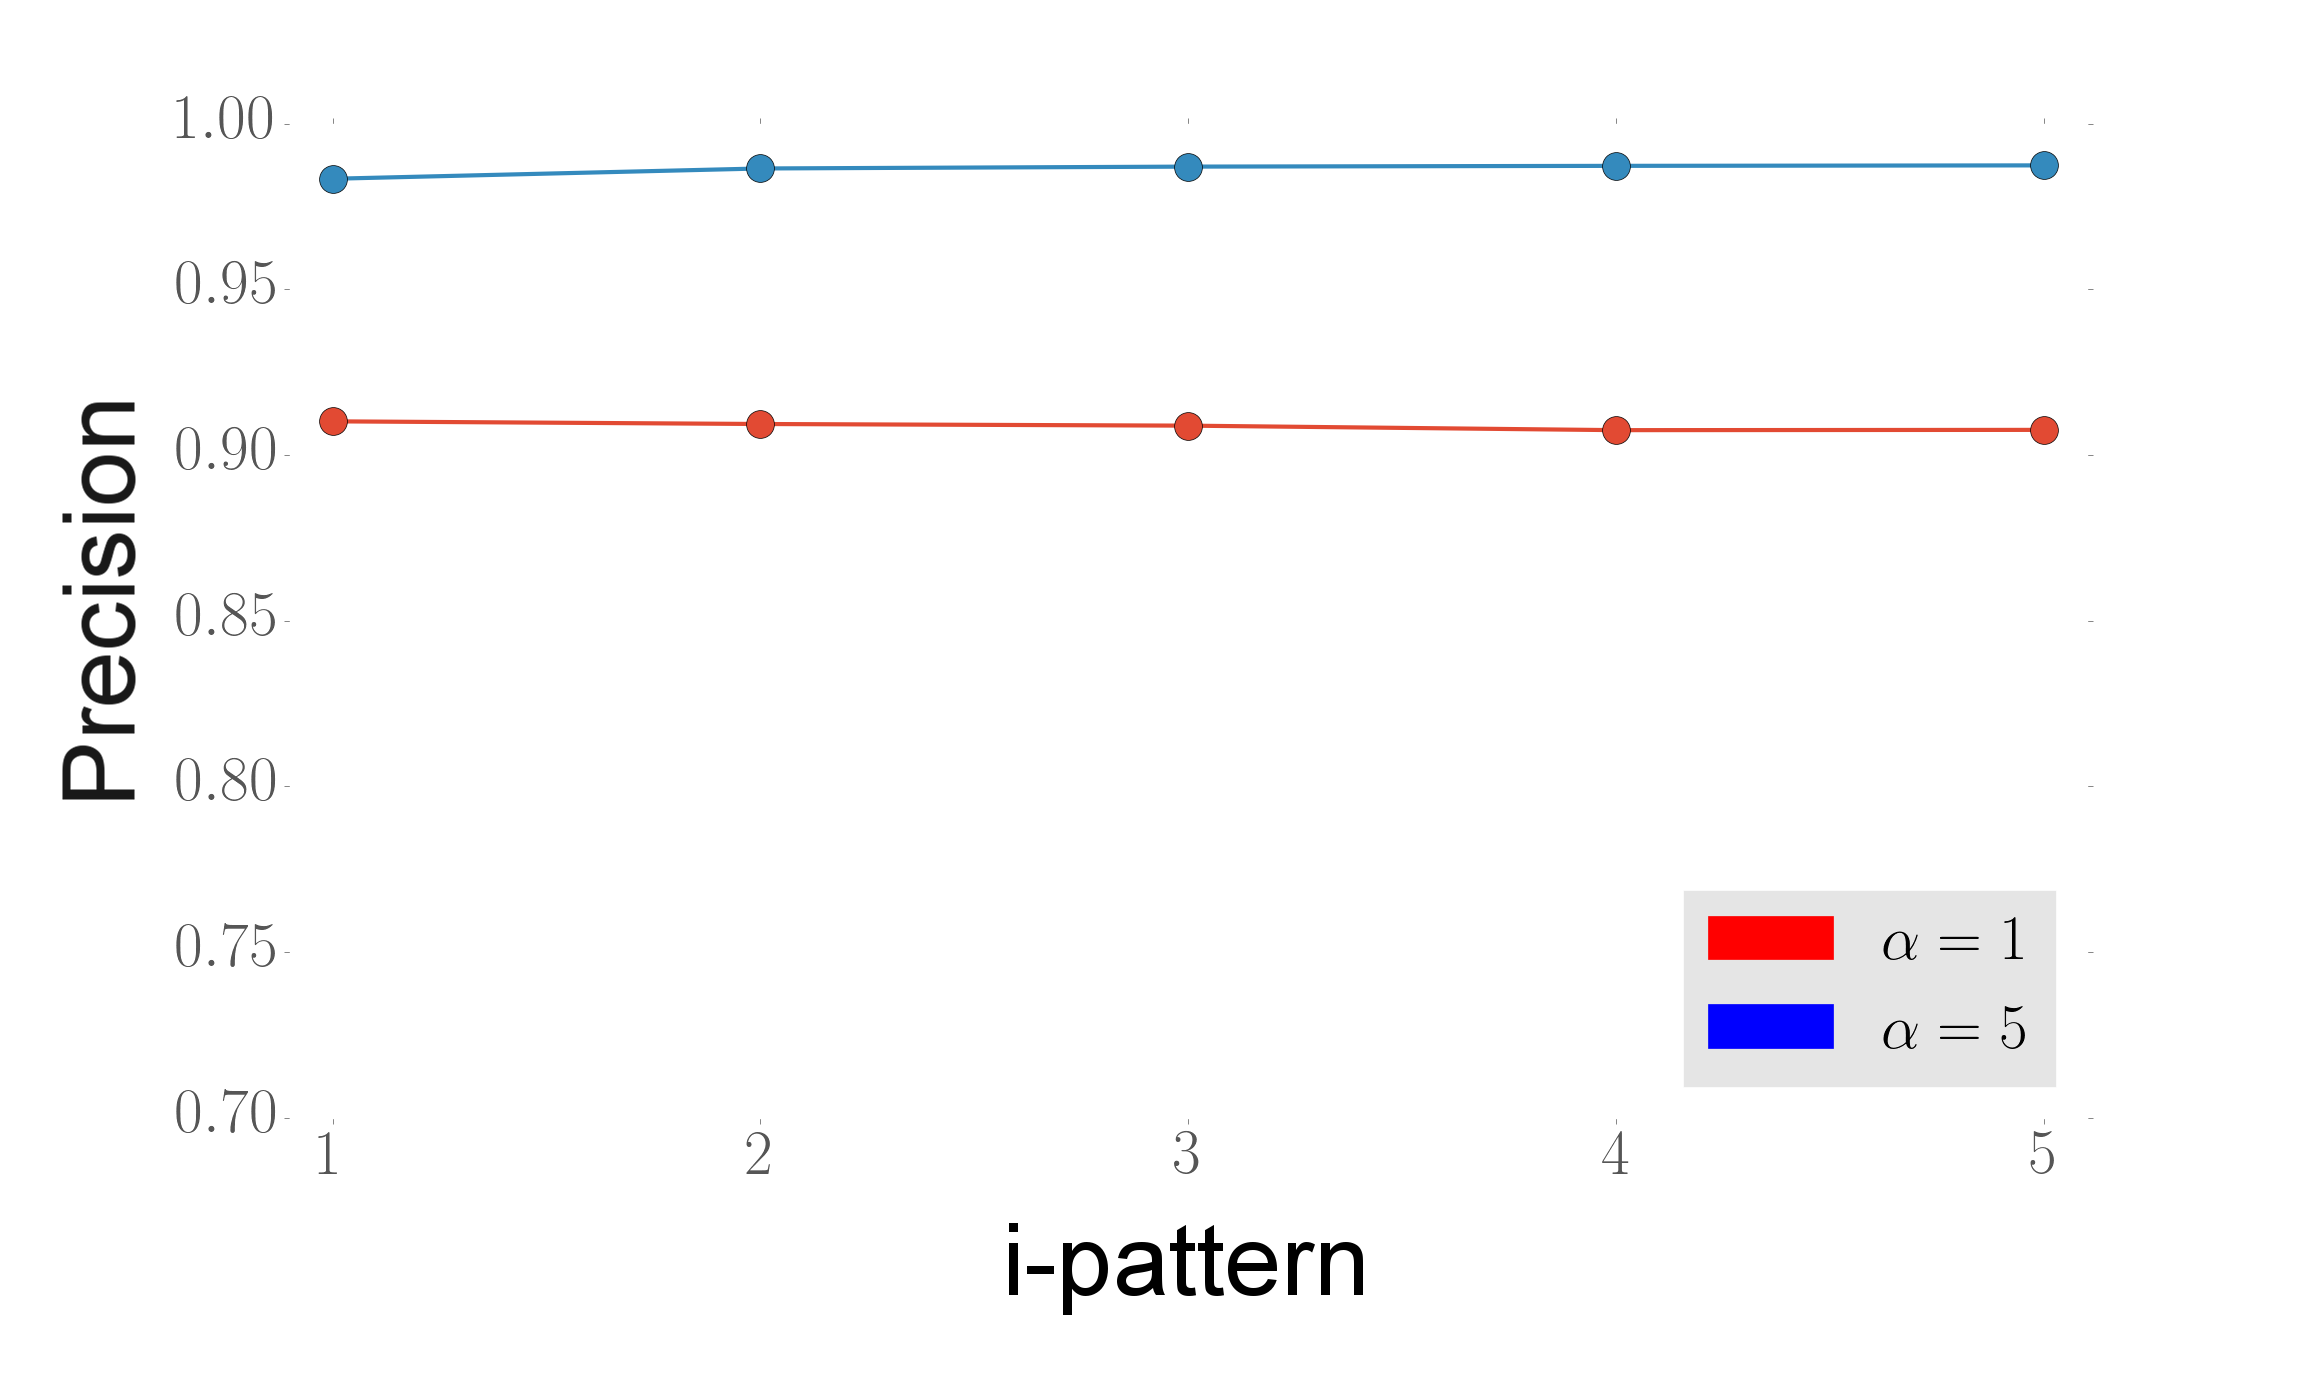
\includegraphics[width=\textwidth]{discriminative_precision_relational.png}
  \caption{Precision}
\end{subfigure}
   \hfill 
\begin{subfigure}{.49\textwidth}
  \captionsetup{skip = 2pt}
  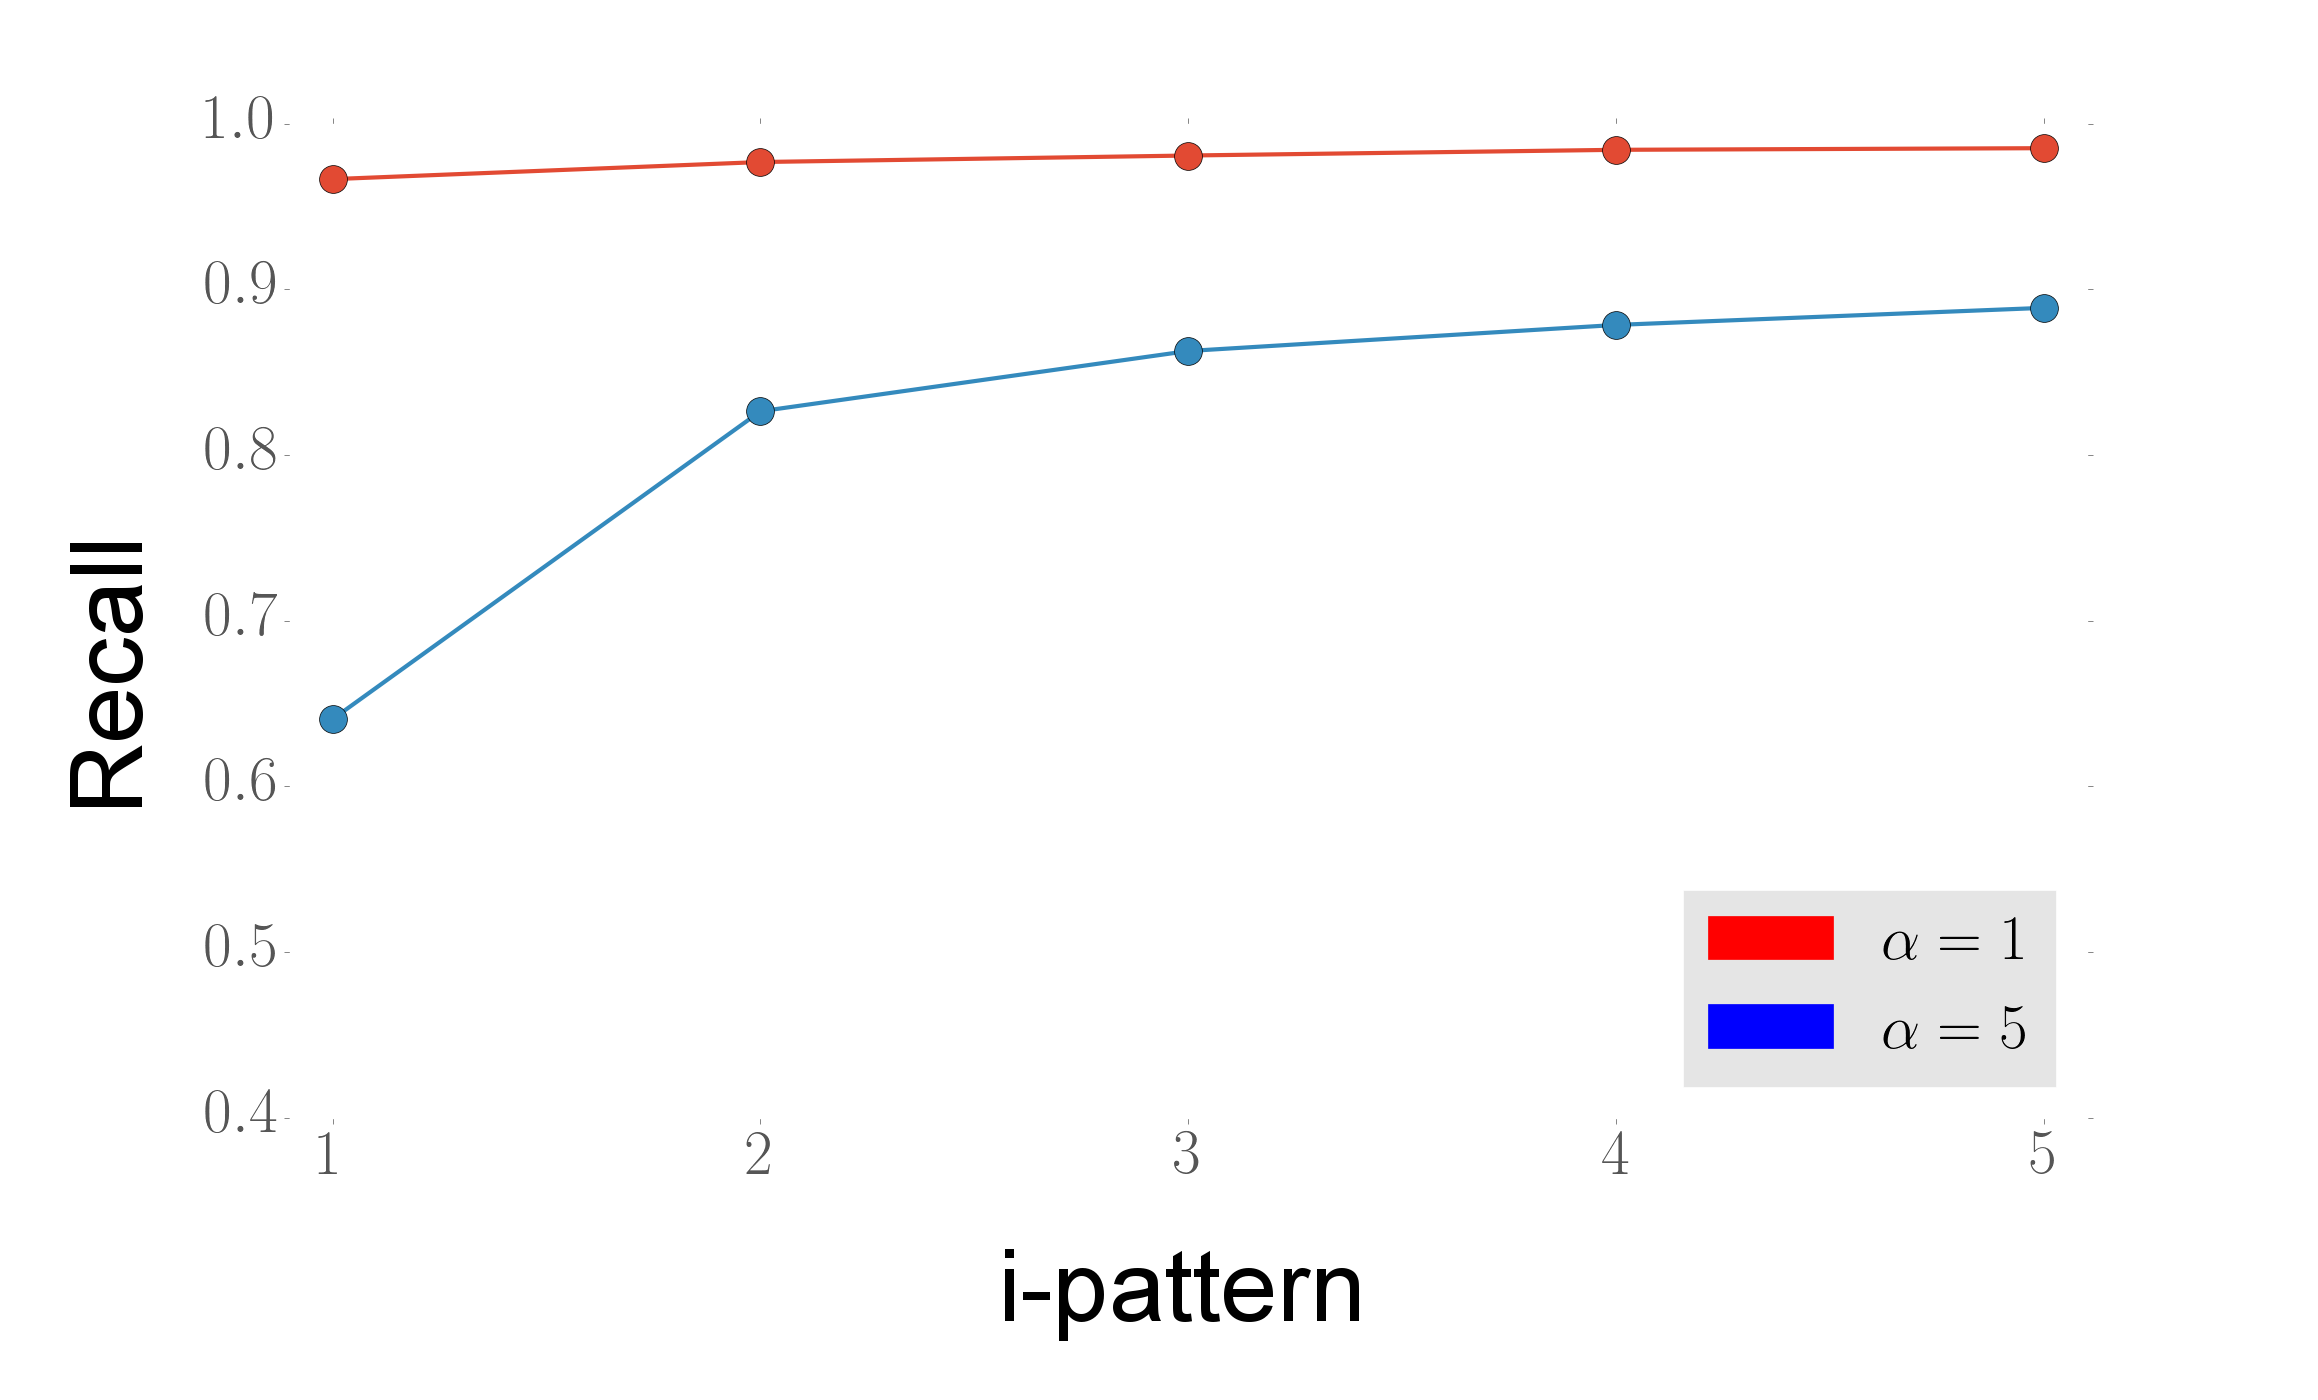
\includegraphics[width=\textwidth]{discriminative_recall_relational.png}
  \caption{Recall}
 \end{subfigure}
 \end{center}
  \captionsetup{skip = -4pt}
  \caption{Discriminative learning in the purely relational setting; precision (left) and recall (right) for different $\alpha$, i.e., for two weights of covering negative atoms.}
  \label{fig:discriminative_precision_recall_relational}
\end{figure}
\subsection{Runtime discussion} 

In this section we have seen a number of experiments that solve ReDF problems using generic solving technology, i.e., answer set programming. As we can see in Figures \ref{fig:tiling_time_comparison} and \ref{figure:bmf}, specialized algorithms are substantially faster than ASP. On datasets of moderate size, however, generic solvers obtain reasonable runtimes, as indicated by the results in Tables \ref{tab:tiling:time}, \ref{tab:overlapping:time}, and \ref{table:discriminative_results}, and Figures \ref{figure:bmf} and \ref{figure:discriminative_chess}. For the purely relational data factorization task from Section \ref{sec:pure_decomposition} we present a summary of the experiments in Table \ref{table:pure}. In these experiments, computation time ranged from several seconds to few minutes.

%Figure \ref{fig:regular_block_diagonal} demonstrates the simplified model from Section \ref{subsec:blockdiagonal}, where instead of constraint \overcoverageConstraint we use \noiseConstraint and we omit the second part (indicated by Eq. \ref{trans_penalty} and \ref{item_penalty}) of optimization function \ref{eq:block_diagonal_optimization}. It does not introduce any penalties for unmatched elements in the same rows and columns as the tile uses, and it does not tolerate presence of the noise in tiles. Figure \ref{fig:penalty_block_diagonal} demonstrates the simplified model from the same section but with penalties, i.e., with the full optimization function. 


